\documentclass[12pt]{article}
\usepackage[utf8]{inputenc}
\usepackage[T1]{fontenc}
\usepackage{geometry}
\geometry{margin=1in}
\usepackage{hyperref}
\usepackage{enumitem}       
\usepackage{apacite}
\usepackage{csquotes}
\usepackage{graphicx}
\usepackage{changepage}
\usepackage[british]{babel}
\usepackage[many]{tcolorbox}
\usepackage{tikzpagenodes}
\usetikzlibrary{tikzmark}
\usepackage{lipsum}
\usepackage[T1]{fontenc}
\usepackage[utf8]{inputenc}
\usepackage{tikz}
\usetikzlibrary{shadows}


\title{GDD (Game Design Document) for A2}
\author{Dylan Rumble-Smith}
\graphicspath{ {./media/} }

\setlength{\parindent}{0pt}
\setlength{\parskip}{1em}

\newtcolorbox{note}[1][]{
	width=\textwidth,
	fonttitle=\bfseries,
	breakable,
	fonttitle=\bfseries\color{Brown},
	colframe=orange,
	colback=orange!10
	#1}


\newcommand*\keystroke[1]{%
	\tikz[baseline=(key.base)]
	\node[%
	draw,
	fill=white,
	drop shadow={shadow xshift=0.25ex,shadow yshift=-0.1ex,fill=black,opacity=0.75},
	rectangle,
	rounded corners=2pt,
	inner sep=1pt,
	line width=0.5pt,
	font=\scriptsize\sffamily
	](key) {#1\strut}
	;
}

\begin{document}
	{\setlength{\parskip}{0pt}%
		\maketitle
		\bibliographystyle{apacite}
		\section*{\centering Abstract}
		\begin{adjustwidth}{90px}{90px}
			This is my Game Design Document for my game named Fringe.
		\end{adjustwidth}
		\pagebreak
		\tableofcontents
		\pagebreak
		}
	
	\section{Introduction}
	In this document, I aim to explain the processes and logic behind the artifacts for my A2 project, while also discussing the culture and history of other games and genres. Additionally, I'll review video game laws and how developers and publishers adapted to them when releasing games.
	
	This document is to be used along with a copy of my video game, as this document will refer to mechanics within that game and explain the context and inner-workings of them.
	\subsection{Game Title}
	The title of the game I am making is Fringe, stylised as FRINGE in promotional material. The title of my game is directly related to its definition, as the word “fringe” is defined as:
	\begin{displaycquote}{fringeMirriamWebster}
		something that is marginal, additional, or secondary to some activity, process, or subject
	\end{displaycquote}
	
	One reason I picked this name is the similarity to the word fling, which promptly explains that within my video game, Fringe, the player is expected to fling themselves off walls and other surfaces within a region nearby them.
	
	Another reason I called the game Fringe is because of the other definition of the word fringe:
	\begin{displaycquote}{fringeMirriamWebster}
		something resembling a fringe: EDGE, PERIPHERY
	\end{displaycquote}
	
	This ties into the story of the game as the character is on the fringe of the law and has to be kept in check.
	
	\subsection{Genres, Subgenres, and Inspiration}
	To make it easy for consumers to find a game that they are seeking, like songs and TV, video games can also be sorted into genres and subgenres. Common genres include, but are not limited to, action games, adventure games, puzzle games, and simulation games.
	
	These genres also have subgenres as well; for example, subgenres for the action genre may include platformer games, shooter games, fighting games, and survival games. These subgenres allow for more specific labelling of games.
	\newpage
	One game I am inspired by is Mirror’s Edge: A video game released in 2008. The game follows the main character Faith, a runner in the society of Mirror’s Edge. These runners carry sensitive documents with them and act as a courier. \cite{mirrorsEdgeGamespot}
	
	The game is labelled as an action adventure game, which is a type of action game. This means that it has action, and it has an adventurous theme.
	
	\begin{figure}[h]
		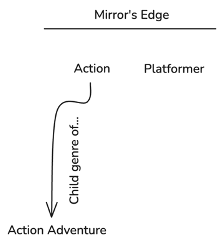
\includegraphics{mirrorsEdgeGenres}
		\centering
		\caption{A diagram showing the genres of Mirror's Edge}
	\end{figure}
	
	Mirror’s Edge has numerous mechanics that it is famous for, such as wall jumping and wall sliding. These mechanics allow for adding complexity to the level design and make the game more interesting as the player can do more actions to complete a level.
	
	For my game I would model my game towards the platformer genre and the action genre.
	
	\subsection{Platforms}
	I am planning to build my video game for the x64 CPU architecture for Windows and the x64 CPU architecture for Linux. Though Linux can run Windows executables through the \href{https://www.winehq.org}{Wine} translation layer, I'd like to also expermiment with making builds for Linux as well.
	
	I am not planning on releasing my game with VR support or mobile support as it would be too time consuming to add support for these, as both of these input devices are very different from the one im targeting (Keyboard and Mouse).
	
	\newpage
	\subsection{Target Audience}
	My target audience is someone who is interested in parkour and action games. From my research, they are 13.6\% more likely to be male, \cite{gameTreeIndustryReports} from the US, \cite{gameDiscoverCoCountryBreakdown} and owns a computer with the specifications of:
	\begin{itemize}
		\item Windows 11.
		\item 16GBs of RAM.
		\item A 6-Core CPU with a clock speed of 2.495GHz.
		\item An NVIDIA GeForce RTX 3060 GPU with 8GBs of VRAM.
	\end{itemize} \cite{steamHardwareSurvey}
	
	\section{Game play and Mechanics}
	\begin{note}
		\textbf{Note:} Due to an unexpected cyber attack against the school network, essential services were down. These services being down caused students to lose the ability to do their school work. To make up for this, the games department reduced the scope of the brief to one where you only have to make the level. So, many of the mechanics are missing from the build of the game. The mechanics listed here were the \textbf{proposed} mechanics before any idea of a cyber attack.
	\end{note}
	\subsection{Gameplay Loop}
	The gameplay loop consists of doing a parkour level and being brought back to the start if the player has hit a fail condition (E.g. the player jumped of a surface) or if the player has decided to reset the level through a GUI. This repetition of playing the same course over and over again until their successful final run gives the player fulfillment once they have finished their final run.
	\newpage
	\subsection{Controls}
	The controls are pretty simple and most mechanics are done automatically as the user plays the game.
	
	\begin{figure}[h]
		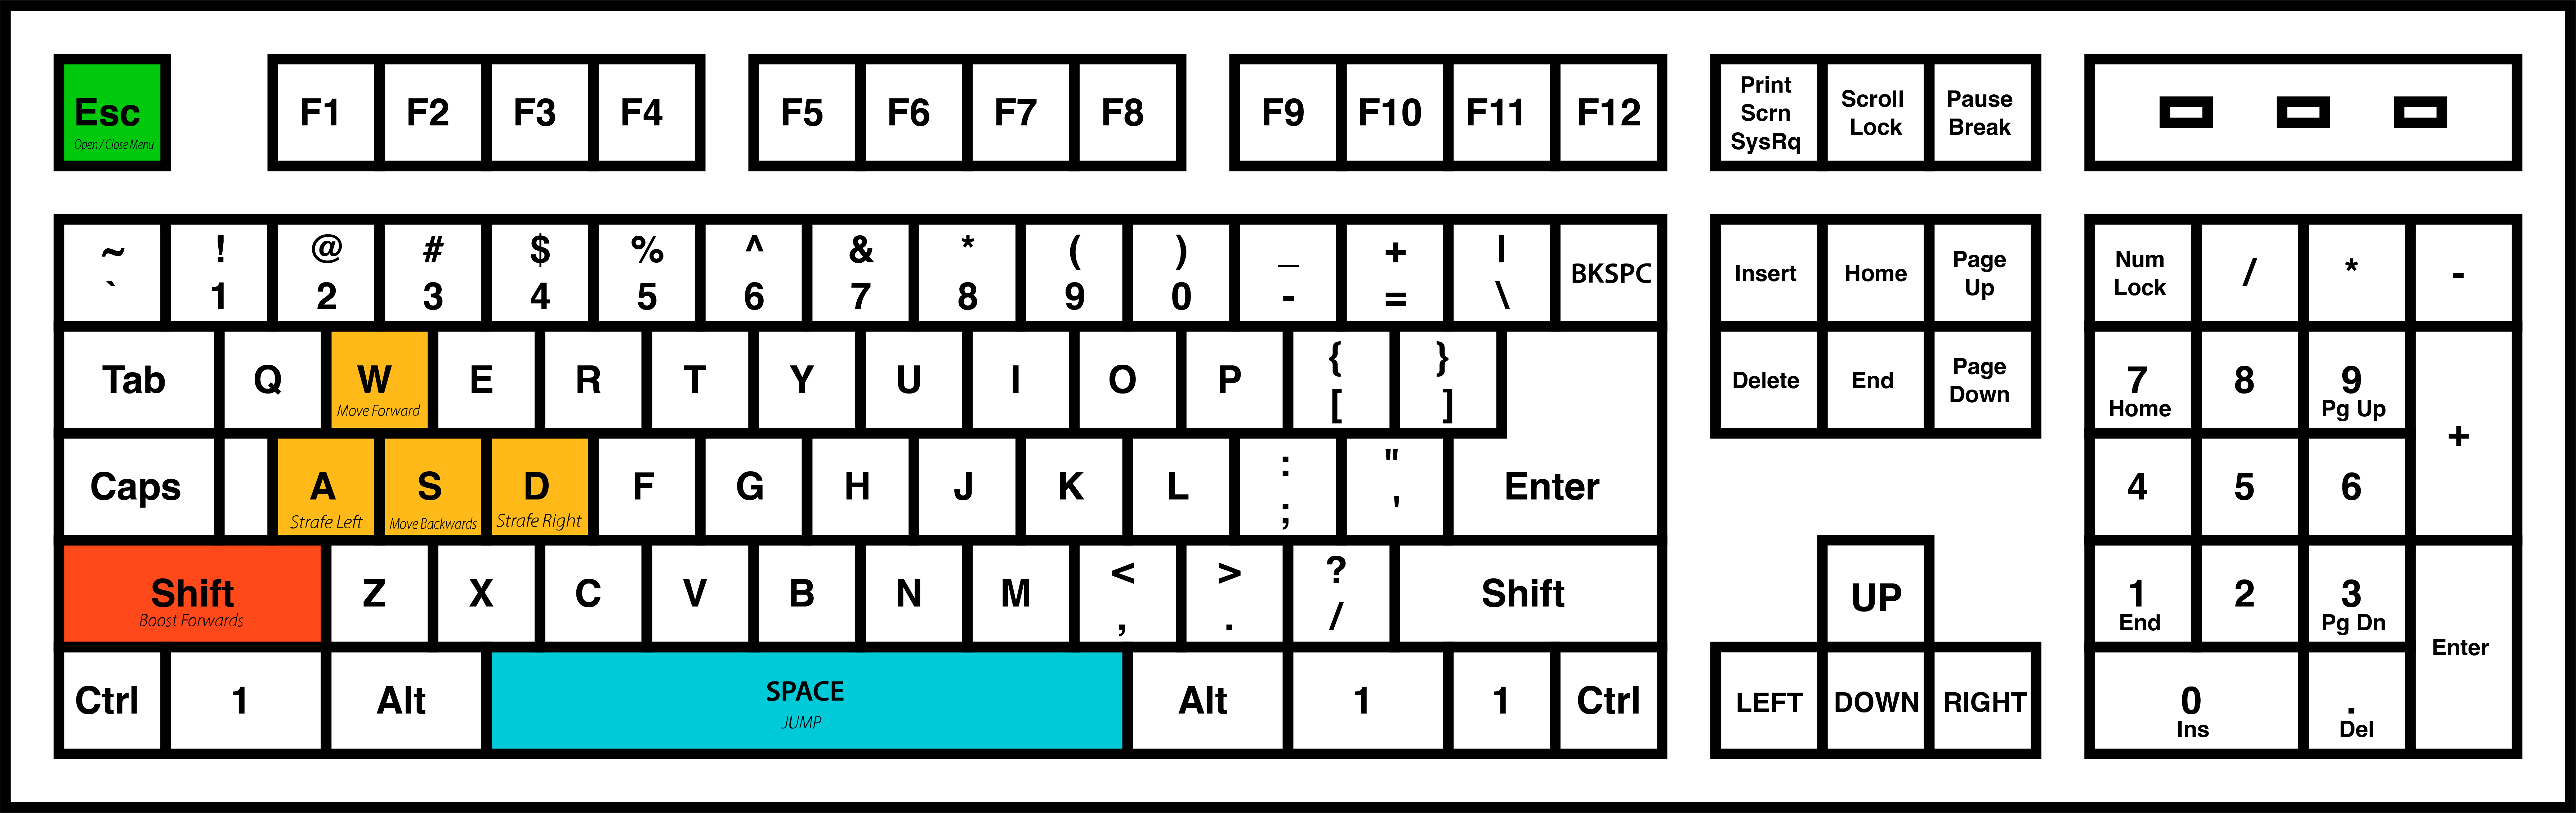
\includegraphics[scale=0.2]{keyboardLayout}
		\centering
		\caption{An annotated keyboard with the specific actions shown on each key}
	\end{figure}
	
	I am not planning to add controller support into the game.
	
	\subsection{Player Abilities}
	The player has multiple abilities (bar the regular movement):
	\begin{itemize}[]
		\item Boost \keystroke{SHIFT} - The player can add some momentum in the air by hitting the \keystroke{SHIFT} key. This, along with a jump, via the \keystroke{SPACEBAR} key, propels the player further.
		\begin{figure}[h]
			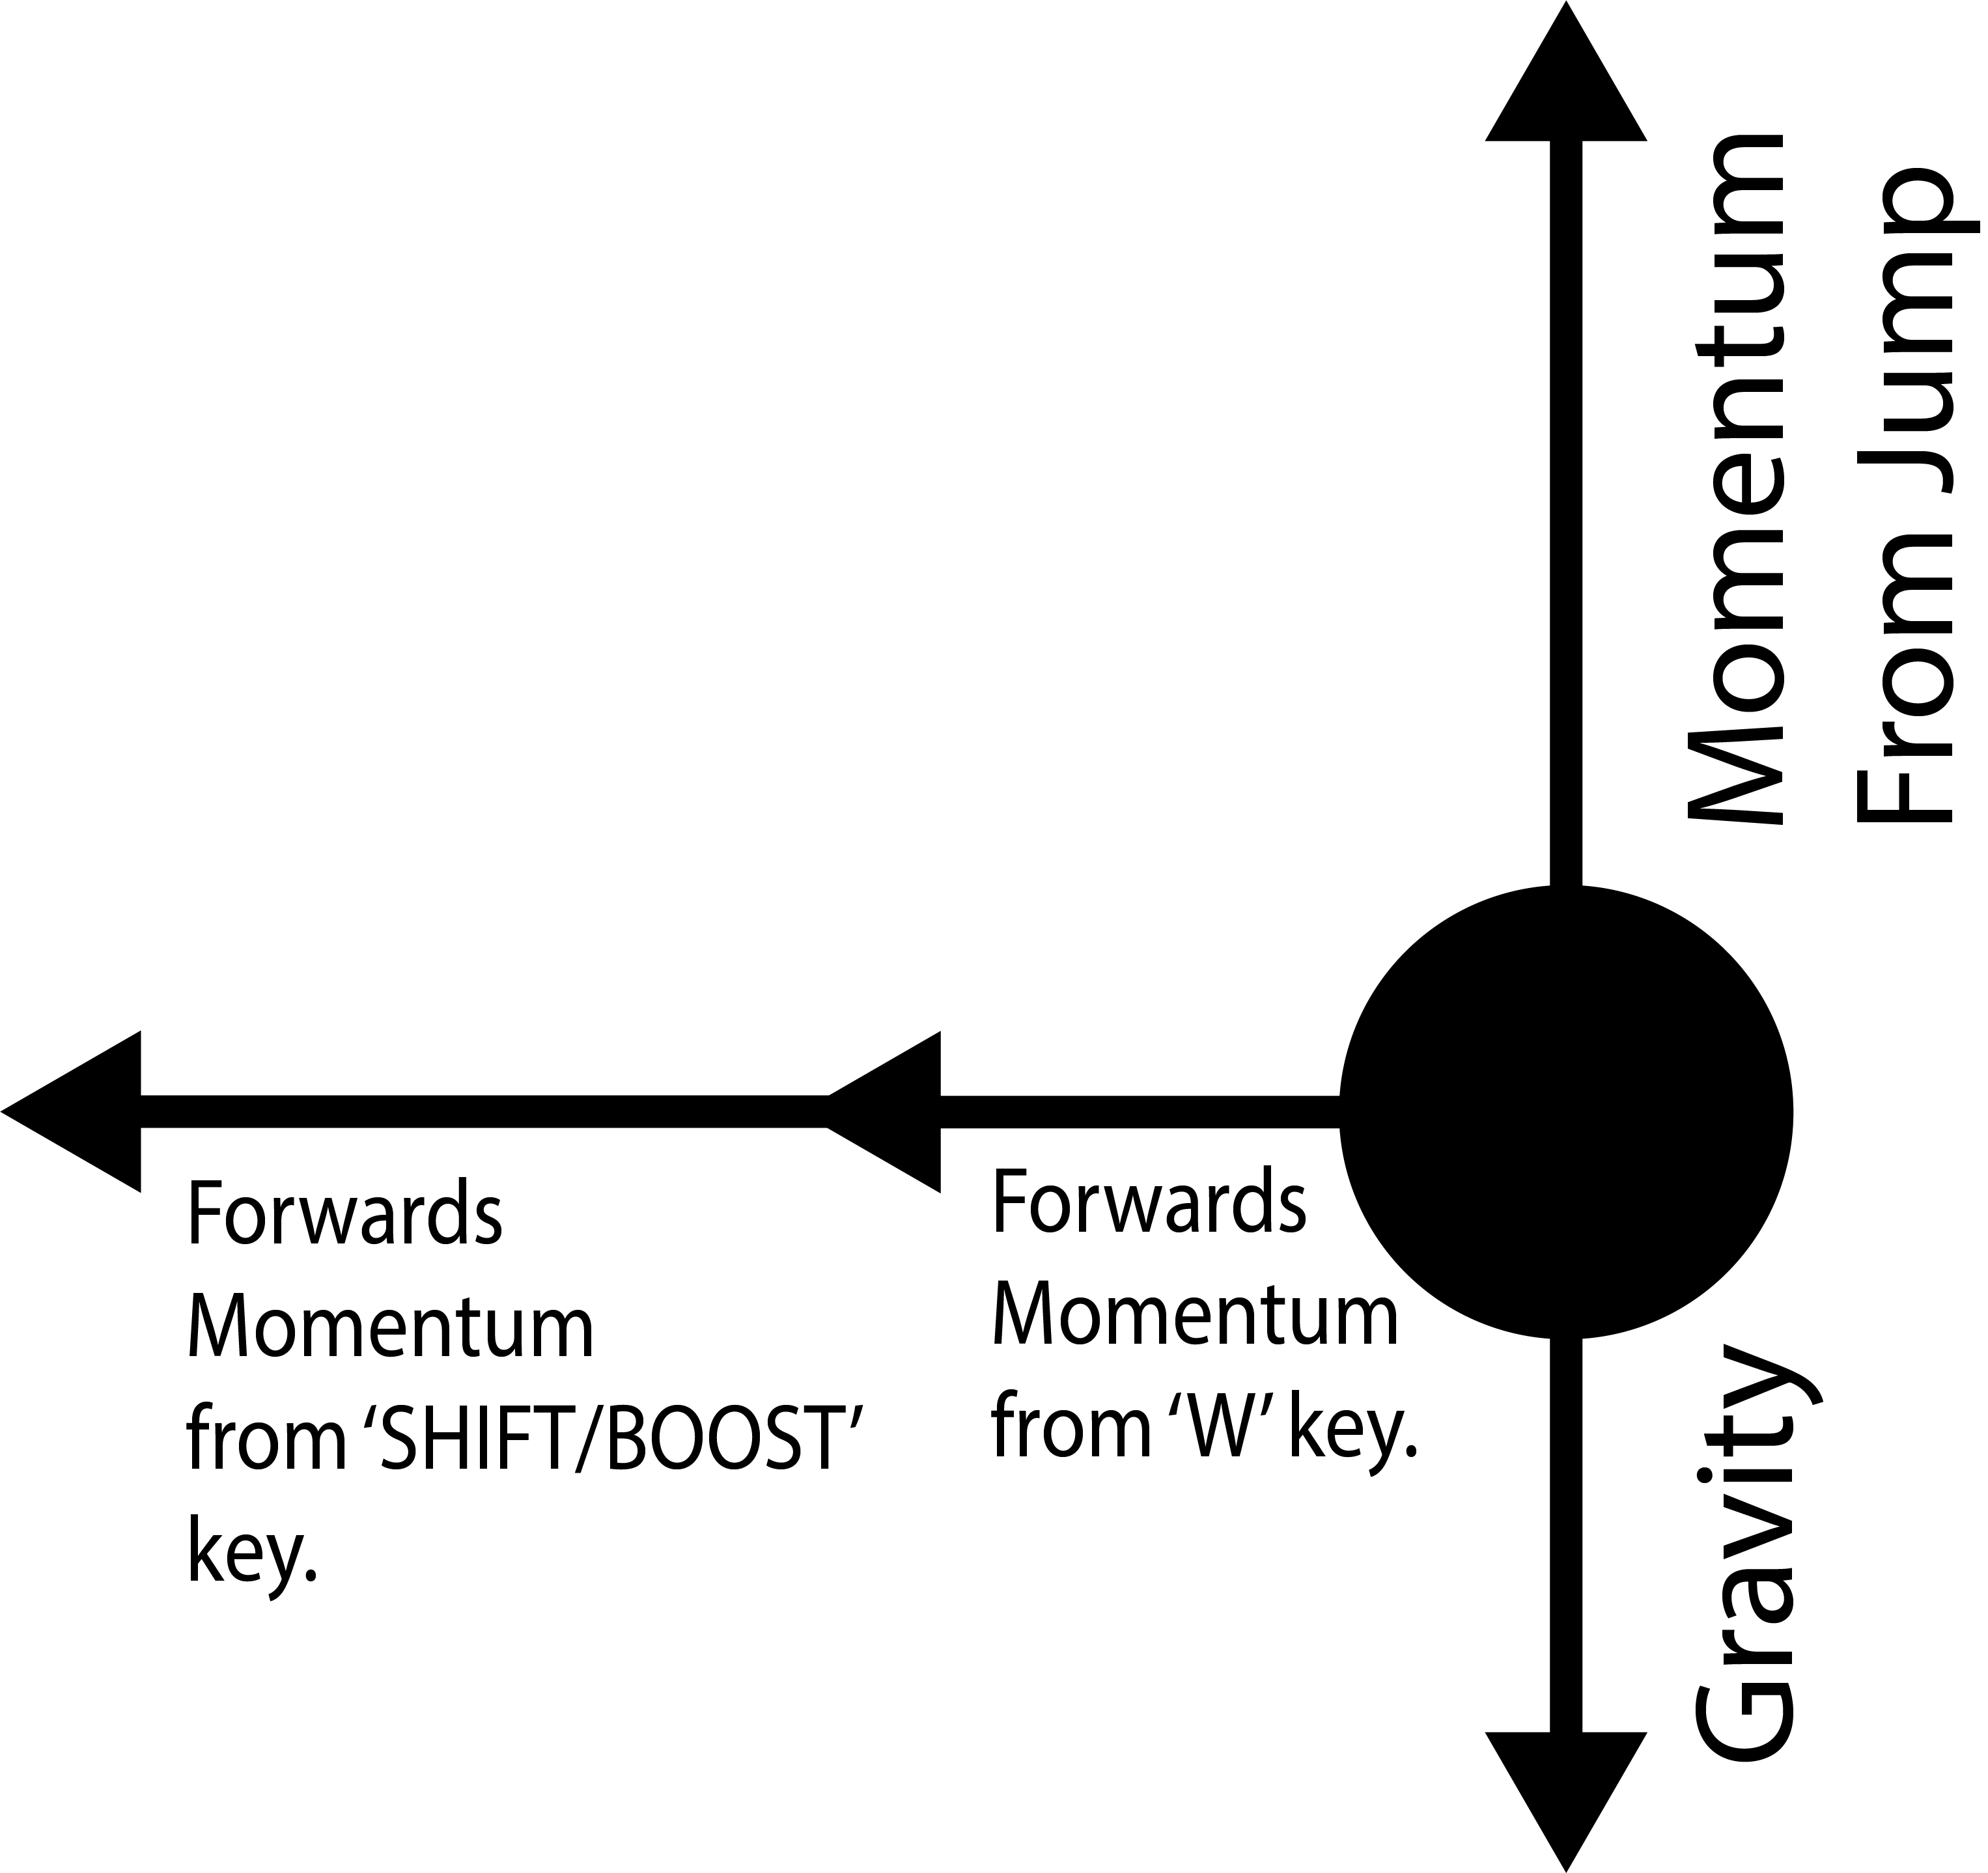
\includegraphics[scale=0.2]{jumpAndBoostForces}
			\centering
			\caption{The forces that are applied on the player when they jump and use the boost mechanic at the same time}
		\end{figure}
		\newpage
		\item Sliding \keystroke{N/A} - The slide mechanic allows for players to pick up speed along downward slopes. The player can use their mouse to control the direction of the slide. Sliding only works if the angle is in a goldilocks zone of angles.
		\begin{figure}[h]
			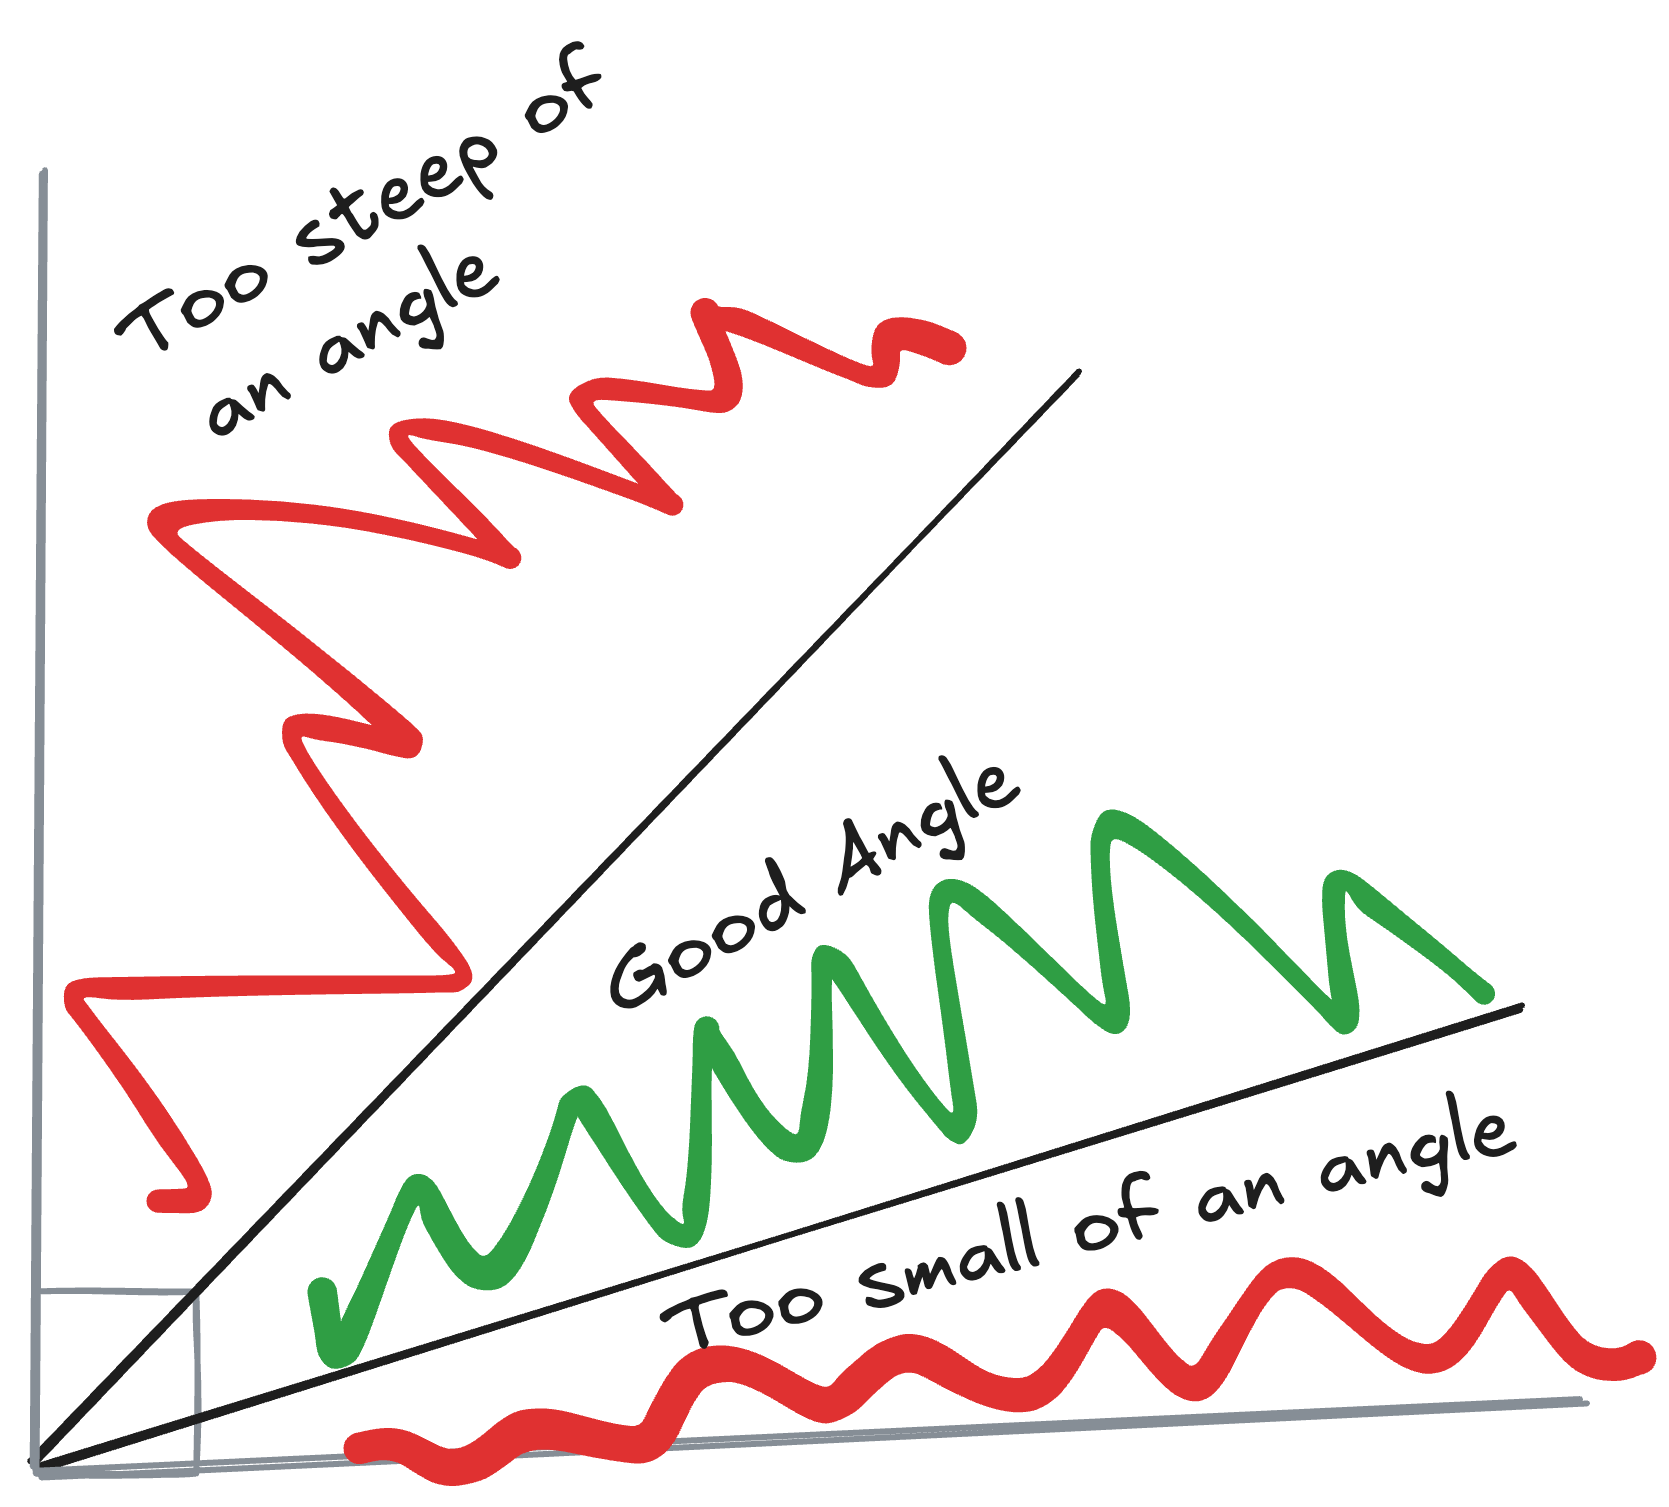
\includegraphics[scale=0.1]{angleSteepness}
			\centering
			\caption{A diagram showing "good angles" and "too steep / small of an angle".}
		\end{figure}
	\end{itemize}

	\subsection{Difficulty and Progression}
	The games difficulty is more or less constant, bar the tutorial, the game sits at a medium difficultly. If the game is too easy, it would not feel as good when the player completes a level and, if it is too hard, the player will feel frustrated.

	There are a number of variables that I could use to change difficulty:
	\begin{itemize}
	  \item The walk speed.
	  \item The amount of time that the Boost mechanic takes to regenerate.
	  \item The spacing between platforms.
	  \item The amount of speed that sliding down a surface generates.
	\end{itemize}

	\section{Level and World Design}
	I was planning on creating multiple levels, however, as previously mentioned, the school network being down got in the way of a few things. So, instead, I am only planning on creating one.
	Here is a list of the levels / worlds I was planning on making:
	\begin{itemize}
	  \item Main Menu (Although this level is not meant to be actually played and enjoyed, it would still be a world.)
	  \item Level 1: Desert (This is the one I am planning on actually making, since it's easily doable to make in a small time-frame.)
	  \item Level 2: Abandoned Laboratory (This one would take a large amount of time to make. Hence I am not planning on doing it unless I have a large amount of free time.)
	\end{itemize}

	\subsection{Level Structure}
	All levels have a starting point and an ending point. There will be multiple routes to get from the starting point to the ending point. The different routes could expose different parts of the map to the player which would increase player replay ability and would give the player more choice on where to go.


	\newpage
	{\setlength{\parskip}{0pt}%
	\bibliography{references}
	}
	
\end{document}
